\documentclass[12pt]{article}
\usepackage{amssymb} % Para añadir simbolos matematicos
\usepackage{graphicx} % Para añadir imagenes
\usepackage{setspace} % Para modificar espacios entre lineas
\usepackage[left=2.5cm,top=2.5cm,right=2.5cm,bottom=2.5cm]{geometry} % Para establecer el tamaño de los margenes
\author{}
\title{XV Concurso de Programación de la UAM \\ 
"Luis Erick González Moreno" - Solucionario}

\begin{document}
    \maketitle
    \newpage %------------------------------------------------------------------------------------------------------------
    
    \section*{Problema A. Uniendo Puntos}
    \paragraph{}
    \singlespacing
    Este problema consiste en calcular la longitud total, que resulta de sumar las longitudes de las 
    lineas que se forman al unir los puntos de manera consecutiva, es decir $P_{1}$ con $P_{2}$, $P_{2}$ con $P_{3}$, etc;
    hay que tener en cuenta que al llegar al último punto, su siguiente 
    será $P_{1}$, siendo esta la última longitud que sumaremos. El plano es $\mathbb{R}2$, por lo que cada punto será
    dado con sus respectivas coordenadas ($x, y$). En la Figura 1 se aprecian las distintas lineas que se forman al unir los puntos,
    por lo tanto la respuesta es: 
    
    \begin{equation}
        longitud_{total} = \sum_{i=1}^{n} l_{i} \hspace{10mm} 1 \leq i \leq n
    \end{equation}
    \vspace{2mm}

    donde $l_{i}$ es la longitud entre los puntos ($P_{i}$, $P_{i+1}$),
    esta se puede calcular facilmente con la formula para distancia entre 2 puntos, recordemos que $P_{i} = (x_{i},y_{i})$:
    \begin{equation}
        \sqrt{(x_{i} - x_{i+1})^2 + (y_{i} - y_{i+1})^2}
    \end{equation}
    en c++ tenemos una función que nos calcula esto
    la cual es hypot() y recibe como argumentos la diferencia en x y la diferencia en y.
     
    \begin{figure}[h]
        \centering
        \fbox{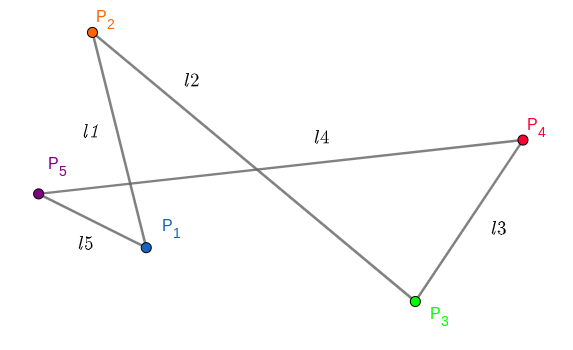
\includegraphics[width=0.4 \textwidth]{problemaA.png}}
        \caption{Lineas que se forman al unir los puntos}
    \end{figure}

    Por último el problema nos pide usar 2 decimales de precisión, esto se puede lograr de la siguiente forma
    \begin{verbatim}
        printf("%.2f", longitud_total); /* para c */
        cout << fixed << setprecision(2) << longitud_total; /* para c++ */
    \end{verbatim}
    Para usar setprecision() hay que añadir en la cabecera a $<$iomanip$>$ y para usar hypot() a $<$cmath$>$.
    
    \vspace{1cm}
    \begin{flushright}
        \textbf{ Complejidad del algoritmo O(n) }
    \end{flushright}

    \newpage %------------------------------------------------------------------------------------------------------------
    
    \section*{Problema B. Super UAMKid Run}
    \paragraph{}
    \singlespacing
    Como queremos minimizar la cantidad de saltos, comenzaremos caminando y avanzaremos hacia la derecha siempre que sea posible,
    ya que cuando nos encontremos un espacio tendremos que forzosamente saltar, cuando lleguemos al espacio en caso de existir
    siempre intentaremos saltar el máximo posible por lo que siempre buscaremos saltar 5, aqui hay varias situaciones:
    
    \begin{itemize}
        \item Si al saltar llegamos al último caracter o lo sobrepasamos (que sería equivalente a saltar menos pero
        justo en el caracter final), hemos terminado.
        \begin{figure}[h]
            \centering
            \fbox{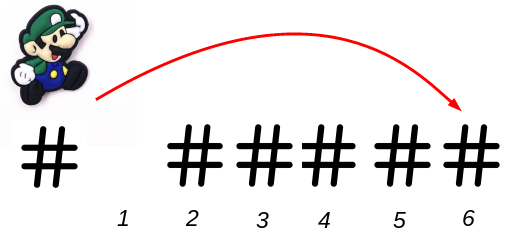
\includegraphics[width=0.3 \textwidth]{uamkid2.png}}
            \fbox{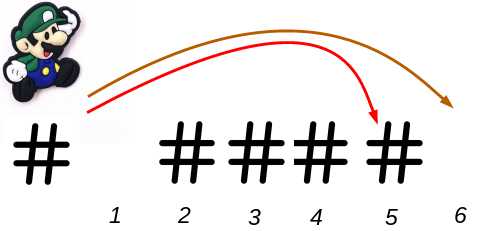
\includegraphics[width=0.287 \textwidth]{uamkid3.png}}
        \end{figure}
        \item Si al saltar llegamos a un espacio entonces tendremos que reducir nuestro salto en 1 hasta que sea \#, ya que 
              tenemos que caer en un \# para poder continuar, en el peor caso nuestro salto será de longitud 1 ya que
              saltaremos únicamente el espacio que encontramos en un inicio.
              Después procedemos a seguir caminando hasta que forzosamente tengamos que volver a saltar o lleguemos 
              al caracter final.
        \begin{figure}[h]
            \centering
            \fbox{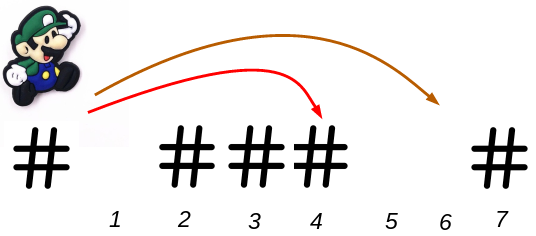
\includegraphics[width=0.3 \textwidth]{uamkid4.png}}
            \fbox{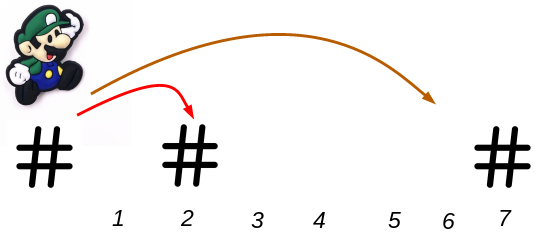
\includegraphics[width=0.3 \textwidth]{uamkid5.png}}
        \end{figure}
        \item Tambien se puede dar el caso de que no sea necesario saltar, ahí la solucion es 0.
    \end{itemize}
    
    \vspace{1cm}
    \begin{flushright}
        \textbf{ Complejidad del algoritmo O(n) }
    \end{flushright}

    \newpage %------------------------------------------------------------------------------------------------------------

    \section*{Problema C. Omitiendo la intersección}
    Hay varias formas de resolver este problema dependiendo de como se manipulen los conjuntos, a continuación se presenta una forma,
    primero encontraremos el conjunto intersección entre A y B al cual llamaremos C, para lograr esto primero ordenaremos ambos conjuntos, de esta forma 
    comparandolos de izquierda a derecha podemos verificar cuales pertenecen a C, c++ tiene una funcion que hace esto,
    set\_intersection(), como más adelante necesitaremos recordar la posición
    original de los elemenos, haremos una copia de los arreglos antes de ordenarlos.    

    \begin{figure}[h]
        \centering
        \fbox{\includegraphics[width=0.4 \textwidth]{problemaC.png}}
        \caption{ Representación de los conjuntos }
    \end{figure}

    \hspace{8mm} El problema nos pide imprimir los elementos que no pertenecen al conjunto intersección según el orden en 
    el que fueron leídos desde la entrada, por esta razón iteraremos sobre nuestra copia del array, es decir el arreglo original.
    Tomamos el primer elemento de izquierda a derecha, y verirficamos si esta en el conjunto C, para evitar la busqueda lineal y que 
    nuestro algoritmo sea lento, podemos usar
    busqueda binaria sobre C o en un inicio utilizar "set" de c++ el cual es un árbol binario balanceado, por lo que
    para saber si un elemento se encuentra con la llamada a sus métodos count o find será suficiente para verificarlo
    esto se hará en $log_{2}$(n) por lo que será eficiente,
    entonces si el elemento es encontrado lo omitimos en caso contrario lo imprimimos.

    \vspace{1cm}
    \begin{flushright}
        \boldmath
        \textbf{ Complejidad del algoritmo O($nlog_{2}n$) }
    \end{flushright}

    \newpage %------------------------------------------------------------------------------------------------------------

    \section*{Problema D. ¿Qué cursos puedo inscribir?}

    \hspace{10mm}Para empezar requerimos separar los requisitos suaves de los duros para cada curso, lo haremos haciendo uso de una
    estructura auxiliar llamada nodo, donde cada nodo consta de un id y de 2 vectores, que representan el id del curso, asi como sus
    requisitos suaves y duros, un vector para cada tipo de requisito. Creando un arreglo de nodos podemos entonces almacenear todos
    nuestros cursos junto a sus requisitos. Como nos solicitan que la salida sea presentada
    en orden, ordenaremos nuestro arreglo de nodos según su id, una vez que ya tenemos ordenados los cursos, iteramos sobre 
    el arreglo, primero verificamos si el curso ya fue aprobado en ese caso no hacemos nada ya que solo nos interesan los que 
    se pueden inscribir, si el curso no ha sido aprobado hacemos lo siguiente.
        

\end{document}